\documentclass[]{article}

% Packages
\usepackage{amsmath} % math stuff
%\usepackage[dvipsnames]{xcolor}  % for coloring
\usepackage{tensor}  % tensors, but also for stuff like superscript on the left
\usepackage{enumitem} % for enumerating alphabetically
\usepackage{tabto}		% for tabbing to a certain length
\usepackage{scrextend} % for local margins
\usepackage{titling}	% for subtitle custom command
\usepackage[svgnames, table]{xcolor} % avoid the option clash for hyperref command  + TABLE REP
\usepackage[colorlinks=true, linkcolor=Blue, urlcolor=Blue]{hyperref} % for hyperref command 
\usepackage{pgfplots} % plots
\usepackage[thinc]{esdiff} % derivative
%%\usepackage{outlines} % convienent itemizing
%%\usepackage{multirow} % multiple rows for tables

%for flowchart:
\usepackage{amsmath}
\usepackage{amssymb}
\usepackage{graphicx}
\usepackage{siunitx}
\usepackage{tikz}
\usetikzlibrary{patterns}
\usepackage{caption}
\usetikzlibrary{arrows}
\usepackage{color}
\usepackage{pgfplots}
\usepackage{listings}
\usepackage[utf8]{inputenc}
\usetikzlibrary{shapes.geometric}
\usepackage{tikz-cd}
\usetikzlibrary{positioning}
\tikzset{
	shift left/.style ={commutative diagrams/shift left={#1}},
	shift right/.style={commutative diagrams/shift right={#1}}
}


%tables for list representation
\usepackage{arydshln, collcell}
\newcolumntype{C}{>{\collectcell\mathsf}c<{\endcollectcell}}

% Python code
\definecolor{codegreen}{rgb}{0,0.6,0}
\definecolor{codegray}{rgb}{0.5,0.5,0.5}
\definecolor{codepurple}{rgb}{0.58,0,0.82}
\definecolor{codeblue}{rgb}{0.08,0.1,0.87}
\lstdefinestyle{pystyle}{
	language=Python,   
	commentstyle=\color{codegreen},
	keywordstyle=\color{codeblue},
	numberstyle=\tiny\color{codegray},
	stringstyle=\color{codepurple},
	basicstyle=\ttfamily\footnotesize,
	breakatwhitespace=false,         
	breaklines=true,                 
	captionpos=b,                    
	keepspaces=true,                 
	numbers=left,                    
	numbersep=5pt,                  
	showspaces=false,                
	showstringspaces=false,
	showtabs=false,                  
	tabsize=2
}
\lstset{style=pystyle}

%Repeat command
\usepackage{expl3}
\ExplSyntaxOn
\cs_new_eq:NN \Repeat \prg_replicate:nn
\ExplSyntaxOff

% Algorithms
\usepackage{algorithm}
\usepackage{algorithmicx}
\usepackage[noend]{algpseudocode}
\newcommand{\Get}{\State \textbf{get}~}
\newcommand{\Set}{\State \textbf{set}~}
\newcommand{\Print}{\State \textbf{print}~}
\newcommand{\Getx}[1]{\Statex \algindent{#1} \textbf{get}~}		% x denotes non-numbered lines
\newcommand{\Setx}[1]{\Statex \algindent{#1} \textbf{set}~}	% enter the number of lines to indent
\newcommand{\Printx}[1]{\Statex \algindent{#1} \textbf{print}~}
\newcommand{\Stop}{\State \textbf{stop}~}
\newcommand{\algindent}[1]{\Repeat{#1}{\hskip\algorithmicindent}}
\algdef{SE}[DOWHILE]{Do}{doWhile}{\algorithmicdo}[1]{\algorithmicwhile\ (#1)}

% plots
\usepackage{pgfplots}
\usepgfplotslibrary{fillbetween}
\pgfplotsset{compat=1.15} 

% stop indentation
\setlength{\parindent}{0pt}

% custom subtitle command
\newcommand{\subtitle}[1]{
	\posttitle{
		\par\end{center}
	\begin{center}\large#1\end{center}
	\vskip0.5em}
}


% Fixes weird backwards quote thing
\usepackage [english]{babel}
\usepackage [autostyle, english = american]{csquotes}
\MakeOuterQuote{"}

% fix upside down exclaimation points for less thans or greater thans
\usepackage[T1]{fontenc}


% Title
\title{PHY 325 Notes}
\subtitle{Computational Physics}
\author{Jaeden Bardati}
\date{\textit{Last modified \today}}

%\setcounter{section}{-1}	% 0-indexes the section

\begin{document}

\maketitle
\bigbreak

\section{Numerical Evaluation of Derivatives}\bigbreak\bigbreak


Let $y = f(x)$, then the \textbf{derivative} is defined as

\begin{equation}\label{eq:limit-definition-of-derivative}
	\diff{f}{x} \equiv \mathop {\lim }\limits_{h \to 0} \frac{{f\left( {x + h } \right) - f\left( x \right)}}{h }
\end{equation}\bigbreak

Now consider $y = f(x_1, ..., x_n)$, then the \textbf{partial derivative} is defined as

\begin{equation}\label{eq:limit-definition-of-partial-derivative}
	\diffp{f}{{x_i}} \equiv \mathop {\lim }\limits_{h \to 0} \frac{{f\left( {x_1, ..., x_{i}+h, ..., x_n} \right) - f\left(x_1, ..., x_n \right)}}{h }
\end{equation}\bigbreak

We can numerically compute derivatives in three main ways: forwards, backwards and with an average of the two.\\

The \textbf{forward} derivative is defined as

\begin{equation}\label{eq:forward-derivative}
	\diff{f}{x} \approx \frac{{f\left( {x + h } \right) - f\left( x \right)}}{h}
\end{equation}\bigbreak

The \textbf{backward} derivative is defined as

\begin{equation}\label{eq:backward-derivative}
	\diff{f}{x} \approx \frac{{f\left( {x - h } \right) + f\left( x \right)}}{h}
\end{equation}\bigbreak

The \textbf{central} derivative is defined as

\begin{equation}\label{eq:central-derivative}
	\diff{f}{x} \approx \frac{{f\left( {x + h } \right) - f\left( x - h \right)}}{2h}
\end{equation}\bigbreak

The smaller $n$ is, the more accurate this approximation is.\\

Note that, while the forward and backward derivatives take the same amount of time to compute, the central derivative has twice the number of calculations to do and so will take longer to run.\\ 

Furthermore, the central derivative can have divergent behaviour. To illustrate this, we can take the central derivative at the point (0, 0) on the absolute value function (see figure \ref{fig:absolute-value}). Notice that the value of the derivative is 0 here, which could lead to undesired effects in the simulations of such systems.\\

\begin{figure}[th!]
	\centering
	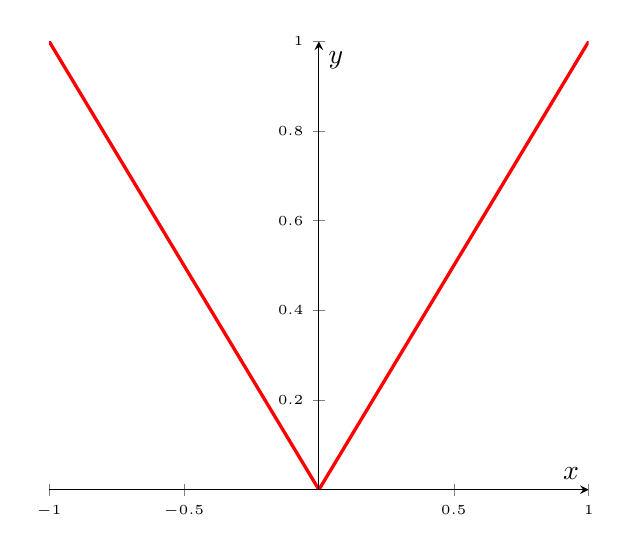
\begin{tikzpicture}
		\begin{axis}[
			axis on top,
			legend pos=outer north east,
			axis lines = center,
			xticklabel style = {font=\tiny},
			yticklabel style = {font=\tiny},
			xlabel = $x$,
			ylabel = $y$,
			legend style={cells={align=left}},
			legend cell align={left},
			]
			\addplot[very thick,red,samples=161,domain=-1:1,name path=f] {abs(x)};
		\end{axis}
	\end{tikzpicture}
	\caption{Absolute value function} \label{fig:absolute-value}
	\bigbreak
\end{figure}

\section{Error in Derivative Calculation}\bigbreak\bigbreak

When implementing a numerical derivative calculation, we would like to use a small value of $h$. But how small? One might think that we should try to make $h$ as small as it can be. Of course, zero will not work since it would result in an error due to division by 0 (see equations \ref{eq:forward-derivative}, \ref{eq:backward-derivative}, and \ref{eq:central-derivative}). \\

If we plot $h$ by the error in the derivative, we will find that the derivative is inaccurate at both high and low values for $h$. There is a "sweet spot" in the middle (roughly around $10^{-8}$) that minimizes the error. The error at low values of $h$ is called \textbf{round-off error} and at high values of $h$ is called \textbf{truncation error}.\\

\subsection{Round-off Error}\bigbreak

To understand this error, we must first ask: How are numbers represented by a computer? Specifically, we are interested in floats. The form is:

\begin{equation}
	s \times M \times B^{e - E}
\end{equation}

where $s$ is the sign (0 if number is positive, 1 if negative), $M$ is the Mantissa, $B$ is the base, $E$ is the bias, and $e$ is the exponent. \\

This form is similar to scientific notation in principle. Namely, it is much more space-efficient to write $1.2 \times 10^{-8}$ rather than 0.000000012. Note that here, 1.2 is the Mantissa, 10 is the base, the sign is 0, and $e-E = -8$.\\

For example, we will look at how 10.75 is stored. In binary, $(10)_{10} = (1010)_{2}$ and $(0.75)_{10} = (11)_2$, where the subscript indicates the base). So, 

\[(10.75)_{10} =  (1010.11)_{2} = (1.01011)_{2} \times 2^3\]\bigbreak

The bias term $E$ is highly dependent on the particular machine you use. However, for a typical 32-bit computer, it is common to have a bias of $E = 2^{n-1} + 1$ with $n=8$. This gives that $E=129$. The base is, of course, $B=2$. \\

Calculating $e$ now, we know

\[e - E = 3 \implies e = 3 + E = 3 + 129 = 132\]\bigbreak

In binary, $(132)_{10} = (10000100)_2$.\\

Therefore, we would store the float value of 10.75 as

\begin{table}[h]\centering
	\begin{tabular}{|c|c|c|}
		\hline
		0 & 10000100 & 10101100000...000\\\hline
		\multicolumn{1}{c}{$s$} & \multicolumn{1}{c}{$e - E$} & \multicolumn{1}{c}{$M$ (23-bits)}
	\end{tabular}
\end{table}

In a 32-bit system, 1 bit is used to store the sign $s$, 8 bits for the exponent $e-E$, and 23 bits for the mantissa $M$. In a 64-bit system (double precision), 1 bit is used to store the sign $s$, 11 bits for the exponent $e-E$, and 52 bits for the mantissa $M$. \\

Since the mantissa is only a certain size, once a decimal value becomes lower than what can be stored in the mantissa, the value is lost. This is round-off error. The machine accuracy for a 32-bit system is around $10^{-8}$ and for a 64-bit system is $10^{-16}$.\\

It is important when analyzing numerical systems to pick normalized units (close to unity). That is to say, choose units such that the numbers that are being used do not have this round-off error effect. \\

\subsection{Truncation Error}\bigbreak





\end{document}
